
Le graphique suivant (Fig.\ref{graph3D}), représentant l'application $\mathcal{W}(a;b)$ appliquée en la fonction (ou signal en 1D) $f=\Pi$ (définie dans la première section de ce dossier) et utilisant l'ondelette mère de Morlet (définie plus haut), illustre la richesse de la transformation en ondelettes continue. \\
A partir d'une ondelette mère, on peut créer une pluralité d'ondelettes "filles" qui vont fournir, par rapport à la transformation classique de Fourier, une plus grande précision dans le traitement des signaux de fréquences constamment changeantes.

\begin{figure}[H]
\centering
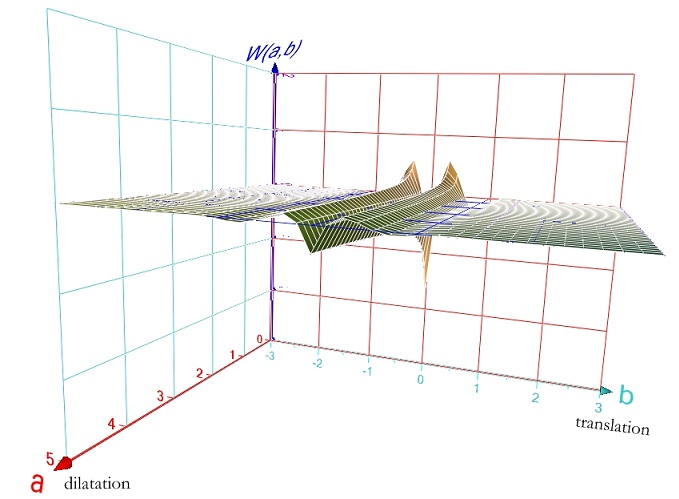
\includegraphics[scale=0.6]{images/graphe3D.jpg}
\caption{Le graphe de la fonction $\mathcal{W}(a;b)(\Pi)$}
\label{graph3D}
\end{figure}

